% !TeX root = trigonometric-functions.tex

\chapter{Analysis of Trigonometric Functions}\label{ch.analysis}

There are two approaches to obtaining the derivative of the trigonometric functions: geometric and algebraic. We will use both approaches to prove that $\sin' x=\cos x$:
\[
\lim_{x \rightarrow 0} \disfrac{\sin (x+h)-\sin x}{h}\stackrel{?}{=}\cos x\,.
\]
In both cases, we need a fundamental concept: as the length of an arc tends to zero, the ratio of the arc to the chord with the same endpoints tends to one.

\section{The ratio of the length of an arc to its chord}

Figure~\ref{fig.arcs-and-chords} shows four arcs and the chords with the same endpoints. The arcs subtend central angles of $80^\circ, 60^\circ, 40^\circ, 5^\circ$. As the arcs get smaller, the difference between the length of the arc and the length of the chord is harder to see. Of course this is what we want, but it is difficult to give an estimate of this difference.

\begin{figure}[hbt]
\begin{center}
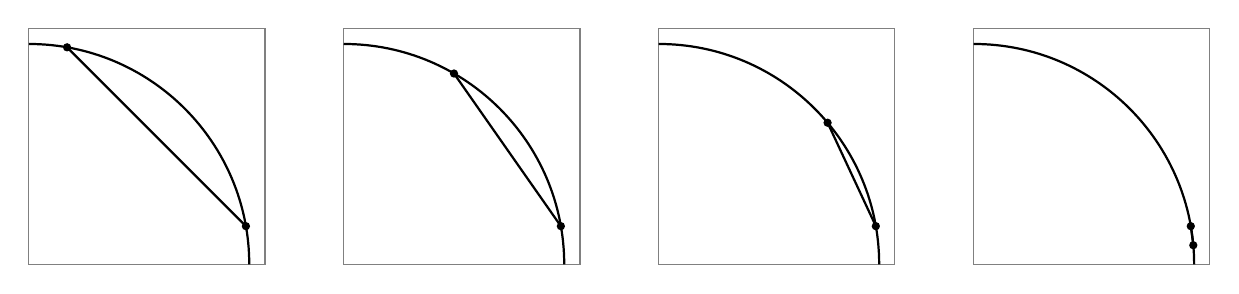
\begin{tikzpicture}
\draw[thin,white!50!black] (0,0) rectangle +(3,3);
\draw[thick] (2.8,0) arc[start angle=0,end angle=90,radius=2.8cm];
\coordinate (s1) at (10:2.8);
\fill (s1) circle (1.5pt);
\coordinate (t1) at (80:2.8);
\fill (t1) circle (1.5pt);
\draw[thick] (s1) -- (t1);
\begin{scope}[xshift=4cm]
\draw[thin,white!50!black] (0,0) rectangle +(3,3);
\draw[thick] (2.8,0) arc[start angle=0,end angle=90,radius=2.8cm];
\coordinate (s2) at (10:2.8);
\fill (s2) circle (1.5pt);
\coordinate (t2) at (60:2.8);
\fill (t2) circle (1.5pt);
\draw[thick] (s2) -- (t2);
\end{scope}
\begin{scope}[xshift=8cm]
\draw[thin,white!50!black] (0,0) rectangle +(3,3);
\draw[thick] (2.8,0) arc[start angle=0,end angle=90,radius=2.8cm];
\coordinate (s3) at (10:2.8);
\fill (s3) circle (1.5pt);
\coordinate (t3) at (40:2.8);
\fill (t3) circle (1.5pt);
\draw[thick] (s3) -- (t3);
\end{scope}
\begin{scope}[xshift=12cm]
\draw[thin,white!50!black] (0,0) rectangle +(3,3);
\draw[thick] (2.8,0) arc[start angle=0,end angle=90,radius=2.8cm];
\coordinate (s4) at (5:2.8);
\fill (s4) circle (1.5pt);
\coordinate (t4) at (10:2.8);
\fill (t4) circle (1.5pt);
\draw[thick] (s4) -- (t4);
\end{scope}
\end{tikzpicture}
\caption{Arcs and the corresponding chords}\label{fig.arcs-and-chords}
\end{center}
\end{figure}
It might be easier to envision the convergence of arcs and chords by examining  regular polygons inscribed within a circle (Figure~\ref{fig.regular-polygons}, \geoproject{g.polygon}).

\begin{figure}[hbt]
\begin{center}
\begin{tikzpicture}
\draw[thin,white!50!black] (-2,-2) rectangle +(4,4);
\coordinate (o1) at (0,0);
\coordinate (a1) at (1.8,0);
\node[draw, name path = circle] at (o1)
    [circle through = (a1)] {};
\foreach \node/\angle in {a2/120,a3/240} {
  \coordinate (\node) at (\angle:1.8);
}
\draw[thick,blue] (a1) -- (a2) -- (a3) -- cycle;
\begin{scope}[xshift=5.5cm]
\draw[thin,white!50!black] (-2,-2) rectangle +(4,4);
\coordinate (o2) at (0,0);
\coordinate (b1) at (1.8,0);
\node[draw, name path = circle] at (o2)
    [circle through = (b1)] {};
\foreach \node/\angle in
  {b2/45,b3/90,b4/135,b5/180,b6/-135,b7/-90,b8/-45} {
  \coordinate (\node) at (\angle:1.8);
}
\draw[thick,blue] (b1) -- (b2) -- (b3) -- (b4) -- (b5) -- (b6) -- (b7) -- (b8) -- cycle;
\end{scope}
\begin{scope}[xshift=11cm]
\draw[thin,white!50!black] (-2,-2) rectangle +(4,4);
\coordinate (o3) at (0,0);
\coordinate (c1) at (1.8,0);
\node[draw, name path = circle] at (o3)
    [circle through = (c1)] {};
\foreach \node/\angle in
  {c2/22.5,c3/45,c4/67.5,c5/90,c6/112.5,c7/135,
   c8/157.5,c9/180,c16/-22.5,c15/-45,c14/-67.5,
   c13/-90,c12/-112.5,c11/-135,c10/-157.5} {
  \coordinate (\node) at (\angle:1.8);
}
\draw[thick,blue] (c1) -- (c2) -- (c3) -- (c4) -- (c5) -- (c6) --
  (c7) -- (c8) -- (c9) -- (c10) -- (c11) -- (c12) -- (c13) --
  (c14) -- (c15) -- (c16) -- cycle;
\end{scope}
\end{tikzpicture}
%\includegraphics[width=\textwidth,keepaspectratio]{figure21}
\caption{Regular polygons inscribed within a circle}\label{fig.regular-polygons}
\end{center}
\end{figure}

The more sides in the polygon, the closer its perimeter is to the circumference of the circle.
The circumference of the circle divided by the number of sides is the length of an arc with the same endpoints as the corresponding side.
(In a regular polygon, all sides have the same length.)
Since the ratio of the circumference of the circle to the perimeter of an inscribed polygon approaches 1 as the number of sides increases, so does the ratio of the length of an arc to the corresponding chord.

To check this numerically, let us compute the length of an arc, the length of the corresponding chord and their ratio.
The length of an arc subtending an angle of $x$ degrees is $2\pi\disfrac{x}{360}$.

%\begin{figure}[H]
\begin{wrapfigure}{r}{.5\textwidth}
\begin{center}
\vspace{-3ex}
\begin{tikzpicture}[scale=1.2]
  \coordinate  (A) at (-2,0);
  \coordinate[label = above left:$O$] (O) at (0,0);
  \fill (O) circle (1pt) node[above right,red,xshift=3pt,yshift=3pt] {$x$};
  \node[draw, name path = circle] at (O)
    [circle through = (A)] {};
  \coordinate (P) at (20:2);
  \fill[red] (P) circle (1.5pt);
  \coordinate (Q) at (70:2);
  \fill[red] (Q) circle (1.5pt);
  \draw[red,very thick] (P)
    arc[start angle=20,end angle=70,radius=2cm];
  \draw[thick,blue] (P) -- node[below left,yshift=2pt] {$c$} (Q) -- 
    node[above left,xshift=2pt] {$a$} (O) -- node[below] {$b$} cycle;
\end{tikzpicture}
\caption{The length of a chord corresponding to an arc of size $x$}\label{fig.length-of-a-chord}
\end{center}
%\end{figure}
\end{wrapfigure}
By the law of cosines the length of a chord $c$ subtending is (Figure~\ref{fig.length-of-a-chord}):
\[
c^2=a^2+b^2-2ab\cos x\,.
\]

In the unit circle $a=b=1$ so:
\[
c=\sqrt{2-2\cos x}\,.
\]
For the arcs and chords in Figure~\ref{fig.arcs-and-chords}:
\[
\begin{array}{|r|r|r|r|}
\hline
\multicolumn{1}{|c}{\textrm{Angle}} &
\multicolumn{1}{|c}{\textrm{Arc length}} &
\multicolumn{1}{|c}{\textrm{Chord length}} &
\multicolumn{1}{|c|}{\textrm{Ratio}}\\\hline
80 & 1.396 & 1.286  & 1.090\\\hline
60 & 1.047 & 1.000  & 1.047\\\hline
40 & 0.698 & 0.684 & 1.006\\\hline
5  & 0.087 & 0.087 &1.000 \\\hline
\end{array}
\]

%\begin{figure}[H]
\begin{wrapfigure}[12]{r}{.5\textwidth}
\begin{center}
\vspace{-3ex}
\begin{tikzpicture}[scale=1.2]
  \draw[thin] (-2,0) -- (2,0);
  \draw[thin] (0,-2) -- (0,2);
  \coordinate[label = above left:$A$]  (A) at (-2,0);
  \coordinate[label = above right:$B$] (B) at (2,0);
  \coordinate[label = above left:$O$] (O) at (0,0);
  \fill (A) circle (1pt);
  \fill (B) circle (1pt);
  \fill (O) circle (1pt) node[above right,xshift=11pt] {$x$} 
    node[below right,xshift=11pt] {$x$};
  \coordinate (P) at (40:2);
  \fill[red] (P) circle (1.5pt) node[above right] {$P$};
  \coordinate (Q) at (-40:2);
  \node[draw, name path = circle] at (O)
    [circle through = (A)] {};
  \draw[red,very thick] (B)
    arc[start angle=0,end angle=40,radius=2cm];
  \draw[red,very thick] (B)
    arc[start angle=0,end angle=-40,radius=2cm];
  \node[red] at (2.1,.8) {$x$};
  \node[red] at (2.1,-.8) {$x$};
  \draw[very thick,blue] (P) -- node[below left] {$\sin x$}
    (P |- O) coordinate (D);
  \draw[very thick,blue] (D) -- node[above left] {$\sin x$} (Q);
%  \fill (D) circle (1pt) node[below right] {$D$};
  \fill[blue] (P) circle (1pt) node[above right] {$P$};
  \fill[blue] (Q) circle (1pt) node[below right] {$Q$};
  \draw (Q) -- (O) -- (P);
\end{tikzpicture}
%\includegraphics[width=.5\textwidth,keepaspectratio]{figure22}
\caption{Ratio of $\sin x$ to $x$}\label{fig.ratio-of-sine-to-x}
\end{center}
%\end{figure}
\end{wrapfigure}

\bigskip

Let us now compute:
\[
\lim_{x \rightarrow 0} \disfrac{\sin x}{x} = \lim_{x \rightarrow 0} \disfrac{2\sin x}{2x}\,.
\]
From Figure~\ref{fig.ratio-of-sine-to-x} we see that this is the ratio the length of the chord $PQ$ to the length of the arc $PQ$.
But we have shown that this ratio converges to $1$ as the subtended angle $2x$ tends to $0$. Therefore:
\[
\lim_{x \rightarrow 0} \disfrac{\sin x}{x} = 1\,.
\]

\bigskip\bigskip\bigskip

\section{The geometric approach}
The limit
\[
\lim_{x \rightarrow 0} \disfrac{\sin (x+h)-\sin x}{h}
\]
is computed by looking at the geometric meaning of each component of the expression.
In Figure~\ref{fig.geometric-computation}, $x$ is the length of the arc from $B$ to $P_x$, $h$ is the length of the arc from $P_x$ to $P_{x+h}$; by adding the arc lengths, $x+h$ is the length of the arc from $B$ to $P_{x+h}$.
Note that the length of an arc in the unit circle is the same as the central angle (in radians) that it subtends.

\begin{figure}[hbt]
\begin{center}
\begin{tikzpicture}[scale=.65]
\coordinate (O) at (0,0);
\coordinate (A) at (0,10);
\coordinate (B) at (10,0);
\fill (O) circle (2pt)
  node[below left] {$O$}
  node[right,xshift=18pt,yshift=6pt] {$x$}
  node[above right,xshift=10pt,yshift=12pt] {$h$};
\fill (A) circle (2pt) node[left] {$A$};
\fill (B) circle (2pt) node[below] {$B$};

\draw[very thick,name path=axes] (B) -- (O) -- (A);
\draw[very thick,name path=arc] (10,0)
  arc[start angle=0, end angle=90, radius=10]
  node[very near start,right] {$x$}
  node[midway,right,yshift=4pt] {$h$};
\draw[very thick,red] (10,0)
  arc[start angle=0, end angle=30, radius=10];
\draw[very thick,blue] (30:10)
  arc[start angle=30, end angle=70, radius=10];

\path[name path=px] (O) -- (30:11);
\path [name intersections={of=arc and px,by={Px}}];
\fill (Px) circle (2pt) node[above right] {$P_x$};

\draw[very thick,name path=pxd] (Px) -- (Px |- O);
\path[name intersections={of=pxd and axes,by={D}}];
\fill (D) circle (2pt) node[below] {$D$};

\path[name path=pxh] (O) -- (70:11);
\path [name intersections={of=arc and pxh,by={Pxh}}];
\fill (Pxh) circle (2pt)
  node[above right] {$P_{x+h}$}
  node[below right,yshift=-10pt] {$\theta$};

\draw[very thick,name path=pxh] (Pxh) -- (Pxh |- O);
\path [name intersections={of=pxh and axes,by={H}}];
\fill (H) circle (2pt) node[below] {$H$};

\draw[very thick,dashed,name path=pxpxh] (Px) -| (Pxh);
\path [name intersections={of=pxh and pxpxh,by={G}}];
\fill (G) circle (2pt) node[left] {$G$};

\draw (D) rectangle +(10pt,10pt);
\draw (G) rectangle +(10pt,10pt);
\draw (H) rectangle +(10pt,10pt);

\draw[very thick,dotted] (O) -- (Pxh);
\draw[very thick,dotted] (O) -- (Px);
\draw[very thick,dashed] (Pxh) -- (Px);

\path (D) -- node[left] {$\sin x$} (Px);
\path (H) -- node[left] {$\sin x$} (G);
\path (G) -- node[left] {$\sin(x+h)\!-\!\sin x$} (Pxh);
\end{tikzpicture}
\caption{Geometric computation of the limit}\label{fig.geometric-computation}
\end{center}
\end{figure}

$P_xD$ and $P_{x+h}H$ are perpendicular to the $x$-axis and $P_xG$ is perpendicular to $P_{x+h}H$.
We are interested in the angle $\theta$, which is the difference between two angles:
\[
\theta=\angle GP_{x+h}P_x= \angle OP_{x+h}P_x - \angle OP_{x+h}H\,.
\]
All radii are equal so $\triangle OP_{x+h}P_x$ is isoceles, and the sum of the angles of a triangle is $\pi$:
\[
\angle OP_{x+h}P_x=\frac{1}{2}(\pi - h)\,.
\]
From the sum of the angles in the right triangle $\triangle OP_{x+h}H$ we have:
\[
\angle OP_{x+h}H = \left(\pi-\frac{\pi}{2}-(x+h)\right) = \left(\frac{\pi}{2}-(x+h)\right)\,.
\]
Therefore:
\[
\theta = \frac{1}{2}(\pi - h) - \left(\frac{\pi}{2}-(x+h)\right) = x+\frac{h}{2}\,.
\]

\smallskip

In the right triangle $\triangle P_xGP_{x+h}$:
\[
\cos \theta = \frac{P_{x+h}G}{P_{x+h}P_x}=\frac{\sin(x+h)\!-\!\sin x}{P_{x+h}P_x}\approx \frac{\sin(x+h)\!-\!\sin x}{h}\,,
\]
taking the length of the arc $h$ as an approximation of the chord $P_xP_{x+h}$. Taking the limit:
\[
\sin' x = \lim_{h\rightarrow 0} \frac{\sin(x+h)\!-\!\sin x}{h} =  \lim_{h\rightarrow 0}\cos \theta = \lim_{h\rightarrow 0} \cos \left(x+\frac{h}{2}\right) = \cos x\,.
\]

\section{The algebraic approach}

We use the identity:
\[
\sin(\alpha) -\sin\beta = 2\sin \frac{\alpha-\beta}{2}\cos \frac{\alpha+\beta}{2}\,,
\]
and the continuity of both the sine and cosine functions:
\begin{eqnarray*}
\lim_{h\rightarrow 0} \frac{\sin(x+h)\!-\!\sin x}{h}&=& \lim_{h\rightarrow 0} \frac{2\sin(\frac{h}{2})\cos(\frac{2x+h}{2})}{h}\\
&=&\lim_{h\rightarrow 0}
  \left[
    \left( 
      \frac{\sin(\frac{h}{2})}{\frac{h}{2}}
    \right)
    \cos\left( x+\frac{h}{2} \right)
   \right]\\
& =& \cos x\,.
\end{eqnarray*}
Students can be asked to justify each of the steps in this computation.

\bigskip

The choice between the two approaches depends on the which skills we wish to reinforce in the students.
Clearly, the geometric approach requires the ability to follow a non-trivial geometric derivation. 
The algebraic approach depends on understanding the concepts of continuity and limits.

We emphasize that both approaches are based on:
\[
\lim_{h\rightarrow 0} \frac{\sin(x+h)\!-\!\sin x}{h} =1
\]
that was proved at the beginning of this chapter.

\bigskip

We refer the reader to the article by Josevich \cite{josevich} who shows how the derivative can be obtained from the principles of classical mechanics.
